\documentclass[12pt,a4paper]{article}
\usepackage[utf8]{vietnam}
\usepackage{amsmath}
\usepackage{amsfonts}
\usepackage{amssymb}
\usepackage{graphicx}
\usepackage{tabularx}
\usepackage{indentfirst}
\graphicspath{{images/}}
\usepackage[margin=2.2cm]{geometry}

\title{\bfseries MỞ RỘNG NGÕ VÀO VỚI IC 74HC165}
\author{Thực hiện: Thi Minh Nhựt -- Email: thiminhnhut@gmail.com}
\date{Thời gian: Ngày 05 tháng 08 năm 2018}

\renewcommand{\arraystretch}{1.3}
\newcommand{\fig}[1]{Hình~#1}
\newcommand{\tab}[1]{Bảng~#1}
\newcommand{\head}[1]{\textbf{#1}}

\begin{document}

\maketitle

\tableofcontents
%
% \pagenumbering{gobble}
%
% \cleardoublepage
%
% \pagenumbering{arabic}

\section{Tìm hiểu về IC ghi dịch 74HC165}
    IC ghi dịch 75HC165 có chức năng mở rộng ngõ vào digital cho vi điều khiển. Có khả năng chuyển dữ liệu ngõ vào từ song song sang nối tiếp và dữ liệu ngõ vào từ nối tiếp sang nối tiếp.

\subsection{Sơ đồ chân của IC 74HC165}
    Sơ đồ chân của IC 74HC165 được trình bày trên \fig{\ref{Fig:Diagram_74HC165}}.
        \begin{figure}[htp]
            \centering
            \fbox{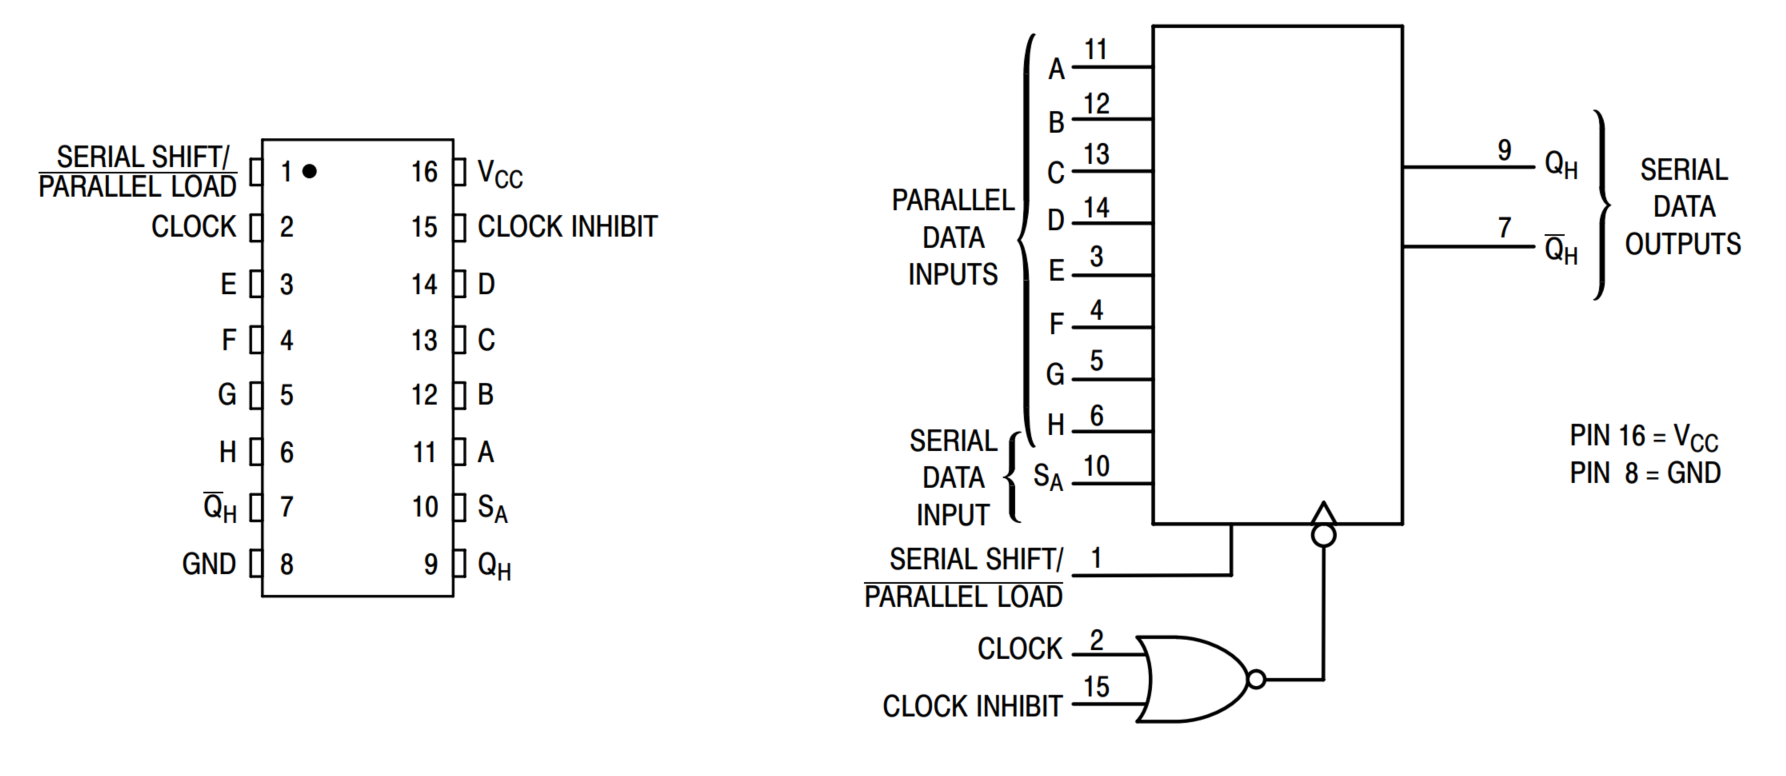
\includegraphics[scale=0.4]{Diagram_74HC165}}
            \caption{Sơ đồ chân của IC 74HC165}
            \label{Fig:Diagram_74HC165}
        \end{figure}

    \newpage
    Chức năng của các chân của IC 74HC165 được mô tả trên \tab{\ref{Tab:Pin_Funtion}}.
        \begin{table}[htp]
            \centering
            \caption{Chức năng của các chân của IC 74HC165}
            \label{Tab:Pin_Funtion}
            \begin{tabular}{|c|m{4.5cm}|m{8.5cm}|}
                \hline
                \head{Nhóm} & \multicolumn{1}{c|}{\head{Ký hiệu chân}} & \multicolumn{1}{c|}{\head{Chức năng}} \\
                \hline
                1 & VCC và GND & Cấp nguồn cho IC hoạt động \\
                \hline
                2 & A -- H & Ngõ vào dữ liệu song song \\
                \hline
                3 & $S_A$ & Ngõ vào dữ liệu nối tiếp (kết nối với IC 74HC165 khác)\\
                \hline
                4 & $Q_H$ và $\overline{Q}_H$ & Ngõ ra dữ liệu nối tiếp (ở trạng thái đảo nhau) \\
                \hline
                5 & SERIAL SHIFT / PARALLEL LOAD &  Chân chốt dữ liệu vào bộ nhớ đệm của IC (chuyển mức tín hiệu từ mức 0 lên mức 1) \\
                \hline
                6 & CLOCK & Mỗi lần tạo xung clock ở chân này (tạo xung clock từ mức 0 lên mức 1) dữ liệu ở ngõ vào lần lượt được đưa đến ngõ ra (bắt đầu từ ngõ vào H), có 8 ngõ vào thì cần tạo 8 xung CLOCK\\
                \hline
                7 & CLOCK INHIBIT & Chân CLOCK INHIBIT ở mức 1 thì không cho phép chân CLOCK xuất dữ liệu ra ngõ ra\\
                \hline
            \end{tabular}
        \end{table}

\subsection{Một số thông số kỹ thuật chính của IC 74HC165}
    Các giá trị điện áp và dòng điện cực đại của IC 74HC165 được cho trên \tab{\ref{Tab:maximum_ratings}} (các giá trị điện áp được so với GND).
        \begin{table}[htp]
            \centering
            \caption{Các giá trị điện áp và dòng điện cực đại của IC 74HC165}
            \label{Tab:maximum_ratings}
            \begin{tabular}{|c|l|c|c|}
                \hline
                \head{Ký hiệu} & \multicolumn{1}{c|}{\head{Tham số}} & \head{Giá trị} & \head{Đơn vị} \\
                \hline
                $V_{CC}$ & Điện áp cấp cho IC & $-0.5 \div 7.0$ & $V$ \\
                \hline
                $V_{in}$ & Điện áp cấp vào các chân dữ liệu & $-0.5 \div V_{CC} + 0.5$ & $V$ \\
                \hline
                $V_{out}$ & Điện áp ra ở các chân dữ liệu & $-0.5 \div V_{CC} + 0.5$ & $V$ \\
                \hline
                $I_{in}$ & Dòng điện trên các chân ngõ vào dữ liệu & $\pm 20$ & $mA$ \\
                \hline
                $I_{out}$ & Dòng điện trên các chân ngõ ra dữ liệu & $\pm 20$ & $mA$ \\
                \hline
                $I_{CC}$ & Dòng điện của nguồn cung cấp cho IC & $\pm 50$ & $mA$ \\
                \hline
            \end{tabular}
        \end{table}

    Các giá trị điện áp mà tại đó IC 74HC165 hoạt động ổn định được cho trên \tab{\ref{Tab:recommended_operating_conditions}} (các giá trị điện áp được so với GND).
        \begin{table}[!htp]
            \centering
            \caption{Các giá trị điện áp mà tại đó IC 74HC165 hoạt động ổn định}
            \label{Tab:recommended_operating_conditions}
            \begin{tabular}{|c|l|c|c|c|}
                \hline
                \head{Ký hiệu} & \multicolumn{1}{c|}{\head{Tham số}} & \head{Min} & \head{Max} & \head{Đơn vị} \\
                \hline
                $V_{CC}$ & Điện áp cấp cho IC & $2.0$ & $6.0$ & $V$ \\
                \hline
                $V_{in}$ & Điện áp cấp vào các chân dữ liệu & $0$ & $V_{CC}$ & $V$ \\
                \hline
            \end{tabular}
        \end{table}

\subsection{Nguyên lý hoạt động của IC 74HC165}
    Nguyên lý hoạt động của IC 74HC165 được trình bày như sau:
    \begin{itemize}
        \item Dữ liệu ngõ vào có 2 dạng, dữ liệu dạng song song hoặc dữ liệu dạng nối tiếp:
            \begin{itemize}
                \item Dữ liệu dạng song song: được đưa vào các chân từ A -- H.
                \item Dữ liệu dạng nối tiếp: được đưa vào chân $S_A$ (lấy dữ liệu từ các IC 74HC165 khác).
            \end{itemize}
        \item Chân SERIAL SHIFT/PARALLEL LOAD chuyển mức tín hiệu từ mức 0 lên mức 1 thì cho phép chốt dữ liệu vào bộ nhớ đệm của IC.
        \item Xuất dữ liệu từ bộ nhớ đệm của IC ra ngõ ra $Q_H$ và $\overline{Q}_H$ khi:
            \begin{itemize}
                \item Chân CLOCK INHIBIT ở mức 0 (chân CLOCK INHIBIT ở mức 1 thì không cho phép xuất dữ liệu ra ngõ ra $Q_H$ và $\overline{Q}_H$ dù có tạo xung CLOCK).
                \item Tạo các xung clock ở chân CLOCK để xuất dữ liệu từ bộ nhớ đệm của IC ra ngõ ra $Q_H$ và $\overline{Q}_H$: bắt đầu từ ngõ vào H lần lượt cho đến ngõ vào A.
            \end{itemize}
    \end{itemize}

\section{Mô phỏng hoạt động của IC 74HC165 trên phần mềm Protues}
\subsection{Mô phỏng hoạt động của IC 74HC165 với ngõ vào song song}
    Sơ đồ mạch mô phỏng: \fig{\ref{Fig:Simulation_74HC165x1}}.
        \begin{figure}[htp]
            \centering
            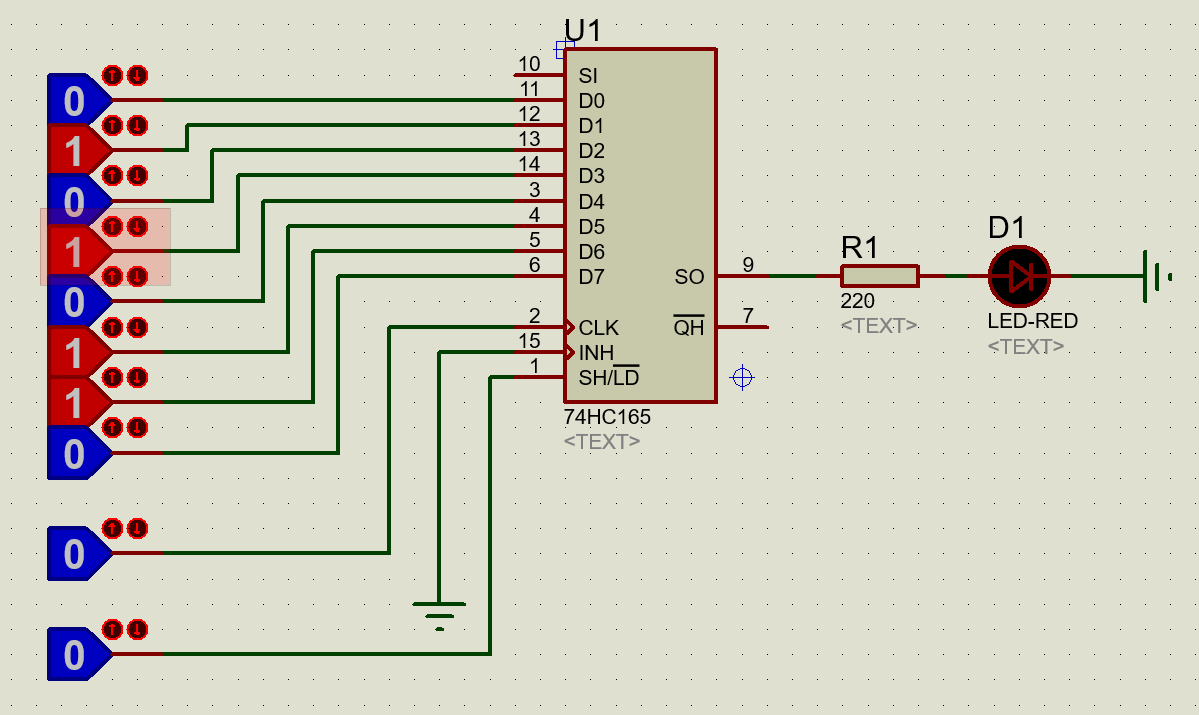
\includegraphics[scale=0.6]{Simulation_74HC165x1}
            \caption{Mô phỏng hoạt động của IC 74HC165 với ngõ vào song song}
            \label{Fig:Simulation_74HC165x1}
        \end{figure}

\newpage

\subsection{Mô phỏng hoạt động của IC 74HC165 với ngõ vào song song và ngõ vào nối tiếp}
    Sơ đồ mạch mô phỏng: \fig{\ref{Fig:Simulation_74HC165x2}}.
        \begin{figure}[htp]
            \centering
            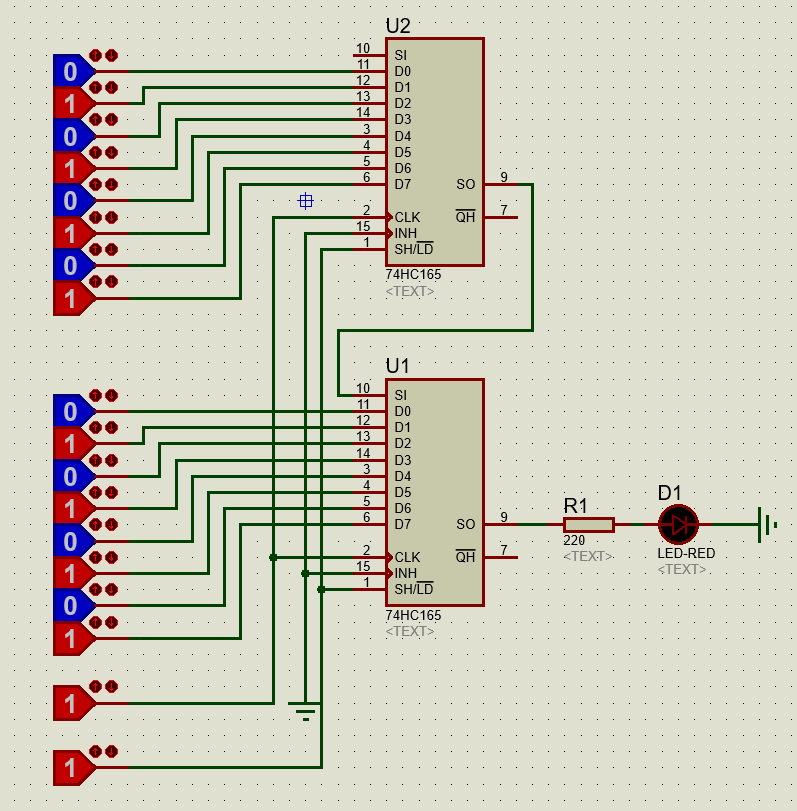
\includegraphics[scale=0.8]{Simulation_74HC165x2}
            \caption{Mô phỏng hoạt động của IC 74HC165 với ngõ vào song song và ngõ vào nối tiếp}
            \label{Fig:Simulation_74HC165x2}
        \end{figure}
\end{document}
